% =====================================================================
%  ESG Report Intelligence - project documentation
%  Overleaf: upload this file, the folder "figures/" and (optionally)
%  "results/prompt_lab_results.tex" exported from the app's Prompt Lab.
%  Compiler: pdfLaTeX (default on Overleaf).
% =====================================================================
\documentclass[11pt,a4paper]{article}

% ---------- fill in your course details ----------
\newcommand{\authorname}{Elsa Shyti}
\newcommand{\coursename}{Generative AI -- Individual Project}
\newcommand{\lecturer}{}            % e.g. Prof. Dr. ...
\newcommand{\githuburl}{}           % e.g. https://github.com/<user>/esg-report-intelligence
% --------------------------------------------------

\usepackage[T1]{fontenc}
\usepackage[utf8]{inputenc}
\usepackage{lmodern}
\usepackage{microtype}
\usepackage[margin=2.3cm]{geometry}
\usepackage{xcolor}
\usepackage{graphicx}
\usepackage{booktabs}
\usepackage{tabularx}
\usepackage{array}
\usepackage{longtable}
\usepackage{float}
\usepackage{caption}

\usepackage{enumitem}
\usepackage{titlesec}
\usepackage{amsmath,amssymb}
\usepackage{listings}
\usepackage{tikz}
\usetikzlibrary{positioning,arrows.meta,shapes.geometric,fit,calc,backgrounds}
\usepackage[most]{tcolorbox}
\usepackage{xurl}
\usepackage{hyperref}

% ---------- colours and layout ----------
\definecolor{navy}{HTML}{1F3864}
\definecolor{esggreen}{HTML}{1F6F50}
\definecolor{esgblue}{HTML}{3A8DBF}
\definecolor{esgamber}{HTML}{E0A526}
\definecolor{esgred}{HTML}{C8423B}
\definecolor{codebg}{HTML}{F4F6F5}
\titleformat{\section}{\Large\bfseries\color{navy}}{\thesection}{0.6em}{}
\titleformat{\subsection}{\large\bfseries\color{navy}}{\thesubsection}{0.5em}{}
\titleformat{\subsubsection}{\normalsize\bfseries\color{esggreen}}{\thesubsubsection}{0.5em}{}
\hypersetup{colorlinks=true,urlcolor=esgblue,linkcolor=navy,citecolor=esggreen,
            pdftitle={ESG Report Intelligence},pdfauthor={\authorname}}
\setlength{\parindent}{0pt}
\setlength{\parskip}{5pt}
\setlist{itemsep=2pt,topsep=3pt}
\captionsetup{font=small,labelfont={bf,color=navy}}
\renewcommand{\arraystretch}{1.15}
\setlength{\emergencystretch}{3em}

\lstdefinestyle{prompt}{basicstyle=\ttfamily\footnotesize,backgroundcolor=\color{codebg},
  frame=single,rulecolor=\color{esggreen!40},breaklines=true,breakatwhitespace=true,
  columns=fullflexible,keepspaces=true,showstringspaces=false,xleftmargin=4pt,xrightmargin=4pt,
  aboveskip=6pt,belowskip=6pt}
\lstdefinestyle{py}{style=prompt,language=Python,keywordstyle=\color{navy}\bfseries,
  commentstyle=\color{esggreen}\itshape,stringstyle=\color{esgred!80!black}}

\newtcolorbox{keybox}[1]{colback=esggreen!5,colframe=esggreen,fonttitle=\bfseries,title=#1,
  boxrule=0.6pt,arc=2pt,left=6pt,right=6pt,top=4pt,bottom=4pt}

% Screenshot macro: shows the image if it exists in figures/, otherwise a placeholder box.
\newcommand{\screenshot}[4][\linewidth]{%
  \begin{figure}[H]\centering
  \IfFileExists{figures/#2}{\fbox{\includegraphics[width=\dimexpr#1-2\fboxsep-2\fboxrule\relax]{figures/#2}}}{%
    \fcolorbox{esggreen}{esggreen!4}{\parbox[c][4.2cm][c]{0.86\linewidth}{\centering\small
      \textbf{Screenshot to add:} \texttt{figures/\detokenize{#2}}\\[3pt]
      Run the app with your Gemini key, take a screenshot of the view described in the caption\\
      and upload it to Overleaf under this file name.}}}
  \caption{#3}\label{#4}\end{figure}}

\newcommand{\code}[1]{\texttt{\small #1}}
\newcommand{\T}{\ensuremath{T}}

% =====================================================================
\begin{document}

% ---------------------------- title page ----------------------------
\begin{titlepage}
\centering
\vspace*{1.6cm}
{\color{esggreen}\rule{\linewidth}{1.2pt}}\\[14pt]
{\fontsize{30}{36}\selectfont\bfseries\color{navy} ESG Report Intelligence\par}
\vspace{8pt}
{\Large A multimodal generative-AI pipeline that turns sustainability reports\\
into verified, traceable ESG data\par}
\vspace{10pt}
{\color{esggreen}\rule{\linewidth}{1.2pt}}\\[30pt]

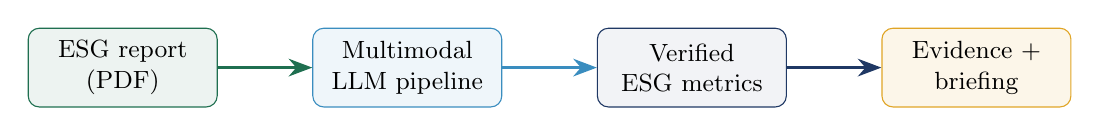
\begin{tikzpicture}[node distance=4mm, every node/.style={font=\small}]
  \node[draw=esggreen,fill=esggreen!8,rounded corners,minimum width=2.4cm,minimum height=1cm,align=center] (pdf) {ESG report\\(PDF)};
  \node[draw=esgblue,fill=esgblue!8,rounded corners,minimum width=2.4cm,minimum height=1cm,align=center,right=12mm of pdf] (ai) {Multimodal\\LLM pipeline};
  \node[draw=navy,fill=navy!6,rounded corners,minimum width=2.4cm,minimum height=1cm,align=center,right=12mm of ai] (data) {Verified\\ESG metrics};
  \node[draw=esgamber,fill=esgamber!10,rounded corners,minimum width=2.4cm,minimum height=1cm,align=center,right=12mm of data] (brief) {Evidence +\\briefing};
  \draw[-{Stealth[length=3mm]},thick,esggreen] (pdf) -- (ai);
  \draw[-{Stealth[length=3mm]},thick,esgblue] (ai) -- (data);
  \draw[-{Stealth[length=3mm]},thick,navy] (data) -- (brief);
\end{tikzpicture}

\vfill
{\large \authorname\par}
\vspace{4pt}
{\coursename\par}
\ifx\lecturer\empty\else{Lecturer: \lecturer\par}\fi
\vspace{4pt}
{November 2026\par}
\ifx\githuburl\empty\else{\vspace{4pt}\url{\githuburl}\par}\fi
\vspace{1.2cm}
\end{titlepage}

% ---------------------------- abstract ----------------------------
\section*{Abstract}
Sustainability reports are long, heterogeneous documents in which the numbers that matter --
greenhouse-gas emissions, water, waste, workforce diversity, supply-chain violations -- are scattered
across running text, tables and charts, and are mixed with targets, baselines and intensities.
\emph{ESG Report Intelligence} is a standalone Streamlit application that uses free generative-AI APIs
(Google Gemini and Groq) to convert such a report into structured, verified ESG data. A user uploads a
PDF; the application parses text, tables and visual content, retrieves the relevant pages with BM25,
extracts 17 standard ESG metrics with a multimodal prompt that combines role prompting, few-shot
examples and chain-of-thought decomposition, repairs malformed output, checks every number against the
PDF with deterministic rules, lets a second ``auditor'' prompt (optionally a second model) verify each
value, and finally writes an analyst briefing. Every figure is traceable: the user can open the source
page with the value highlighted. Sampling parameters are tuned per pipeline stage, a built-in
\emph{Prompt Lab} measures the effect of prompt techniques and temperature, and a layered error-handling
design keeps the application stable under rate limits, timeouts, invalid files and invalid model output.

\tableofcontents
\newpage

% =====================================================================
\section{Introduction}
\subsection{Problem}
Companies publish their environmental, social and governance (ESG) performance in sustainability,
integrated and annual reports. Under the EU Corporate Sustainability Reporting Directive (CSRD) and the
European Sustainability Reporting Standards (ESRS) the volume of such reporting is growing quickly
\cite{csrd,esrs}. Investors, rating agencies and researchers need the reported figures as
\emph{data}: one value per company, metric and year, in a known unit, with a source.

Collecting this data by hand is slow and error-prone. In a previous project the author built a validated
ESG database for a universe of 300 companies from 3{,}421 locally stored report PDFs; even with automated
support, every value had to be checked against its source page. The difficulty is not reading a single
number but \emph{finding the right one}:
\begin{itemize}
  \item values appear in prose, in multi-year tables (often with the scale -- ``kt'', ``thousand m$^3$'' -- only in the header)
        and sometimes \emph{only} in charts;
  \item the same page mixes actual results with targets (``40\,\% women in management by 2028''), baselines,
        intensities and Scope~3 sub-categories;
  \item tables of contents and GRI/ESRS index pages mention every metric but contain no values.
\end{itemize}
Large language models (LLMs) read such material well, but they can also \emph{hallucinate} plausible
numbers. A useful tool therefore has to combine generative extraction with retrieval, verification and
traceability.

\subsection{Objectives}
\begin{enumerate}
  \item Build a working, standalone application with its own front end that solves this real problem end to end.
  \item Use generative AI for substantive multi-step processing -- extraction, classification, verification and
        summarisation -- not question answering.
  \item Process PDFs \emph{multimodally}: text, tables and charts / scanned pages.
  \item Apply and compare several prompt-engineering techniques and tune the sampling parameters per task.
  \item Make every number traceable and every failure mode handled.
\end{enumerate}

\subsection{What the application produces}
For each report the user receives (i) a profile (company, reporting year, report type, frameworks,
assurance), (ii) a table of 17 ConsciESG metrics (optionally 21) with value, unit, standardised value,
year, page, source type, status \textsc{valid}/\textsc{uncertain}/\textsc{invalid}/\textsc{not found} and a
confidence score, (iii) the earlier years reported in the same document as a time series, (iv) per-pillar
disclosure completeness, (v) an evidence view per metric with the PDF page highlighted, (vi) an analyst
briefing with strengths, disclosure gaps and red flags, and (vii) Excel, CSV, JSON and Markdown exports.
All analyses are stored in a local SQLite database.

% =====================================================================
\section{Requirements and how they are met}
Table~\ref{tab:rubric} maps the requirements of the highest grade to the implementation.

\begin{table}[H]
\centering\small
\begin{tabularx}{\linewidth}{@{}>{\raggedright\arraybackslash}p{4.3cm}X>{\raggedright\arraybackslash}p{1.5cm}@{}}
\toprule
\textbf{Requirement} & \textbf{Implementation} & \textbf{Section}\\\midrule
Working standalone application, front end & Streamlit app with 8 tabs, Python back end package \code{esg\_intel} & \ref{sec:ui}\\
API usage & Google Gemini (\code{google-genai}) and Groq (\code{groq}) free tiers, behind one provider interface & \ref{sec:arch}\\
Real-world problem & ESG data extraction from sustainability reports (CSRD/ESRS context) & 1\\
Substantive processing, not Q\&A & 4 LLM stages (profiling, multimodal extraction, verification, summary) + self-repair, retrieval and rule checks & \ref{sec:pipeline}\\
Parameterisation & \code{temperature}, \code{top\_p}, \code{max\_output\_tokens}, thinking/reasoning level, per stage, editable in the UI & \ref{sec:params}\\
$\geq$ 2 prompt techniques & role, zero-shot, few-shot, chain-of-thought decomposition, structured output, self-repair, self-/cross-model verification & \ref{sec:prompts}\\
Experimentation & Prompt Lab: strategies $\times$ temperatures $\times$ repeats, automatic scoring, LaTeX export & \ref{sec:experiments}\\
Error handling & typed error classes, retries with backoff, graceful degradation, input validation & \ref{sec:errors}\\
Extra effort & multimodal input, two providers / cross-model verification, SQLite database, file management, exports, 57 automated tests & \ref{sec:storage}, \ref{sec:tests}\\
Documentation & this document + README & --\\
\bottomrule
\end{tabularx}
\caption{Grading requirements and their implementation.}
\label{tab:rubric}
\end{table}

% =====================================================================
\section{System architecture}\label{sec:arch}
Figure~\ref{fig:arch} shows the architecture. The Streamlit front end only collects settings and displays
results; all processing lives in the \code{esg\_intel} package, which can also be used without the UI
(it is exercised that way by the test suite).

\begin{figure}[H]
\centering
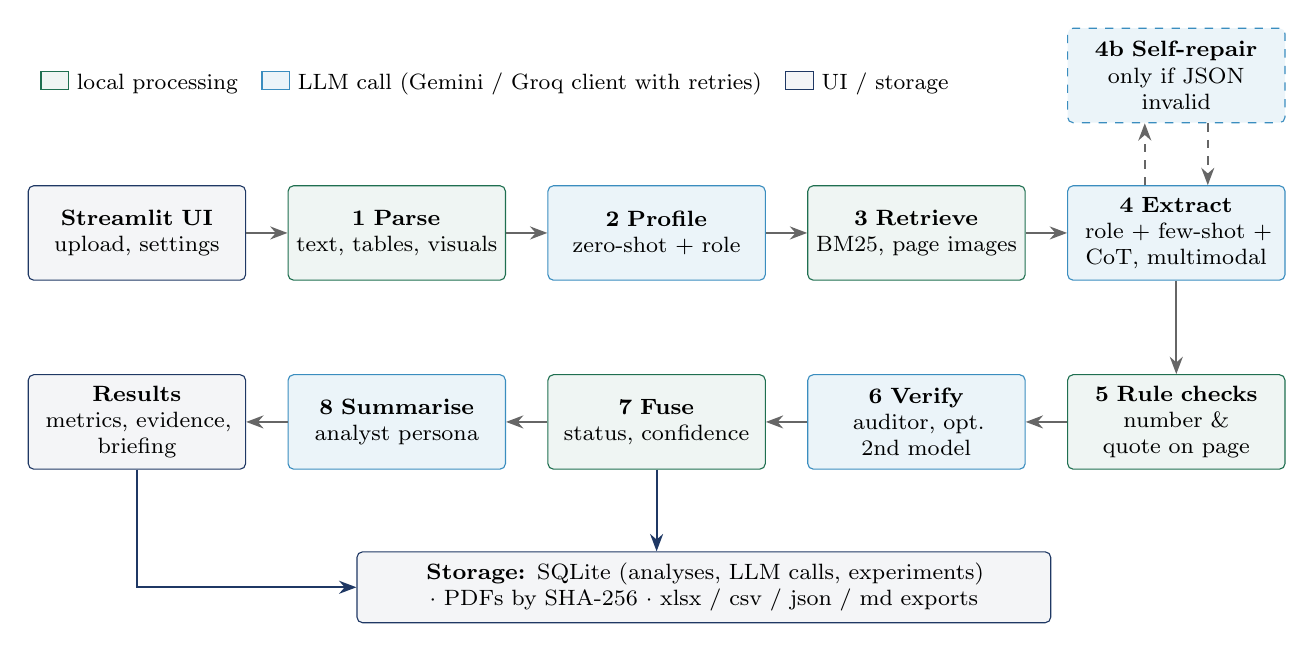
\begin{tikzpicture}[
  every node/.style={font=\footnotesize, execute at begin node={\hyphenpenalty=10000\relax}},
  box/.style={draw,rounded corners=2pt,minimum height=12mm,text width=2.55cm,align=center,inner sep=3pt},
  local/.style={box,draw=esggreen,fill=esggreen!7},
  llm/.style={box,draw=esgblue,fill=esgblue!10},
  store/.style={box,draw=navy,fill=navy!5},
  arr/.style={-{Stealth[length=2.2mm]},thick,color=black!60}]
  % lane 1 (left to right)
  \node[store] (ui)       at (0,0)     {\textbf{Streamlit UI}\\upload, settings};
  \node[local] (parse)    at (3.3,0)   {\textbf{1 Parse}\\text, tables, visuals};
  \node[llm]   (profile)  at (6.6,0)   {\textbf{2 Profile}\\zero-shot + role};
  \node[local] (retrieve) at (9.9,0)   {\textbf{3 Retrieve}\\BM25, page images};
  \node[llm]   (extract)  at (13.2,0)  {\textbf{4 Extract}\\role + few-shot + CoT, multimodal};
  \node[llm,dashed] (repair) at (13.2,2.0) {\textbf{4b Self-repair}\\only if JSON invalid};
  % lane 2 (right to left)
  \node[local] (rules)    at (13.2,-2.4) {\textbf{5 Rule checks}\\number \& quote on page};
  \node[llm]   (verify)   at (9.9,-2.4)  {\textbf{6 Verify}\\auditor, opt.\ 2nd model};
  \node[local] (fuse)     at (6.6,-2.4)  {\textbf{7 Fuse}\\status, confidence};
  \node[llm]   (summary)  at (3.3,-2.4)  {\textbf{8 Summarise}\\analyst persona};
  \node[store] (results)  at (0,-2.4)    {\textbf{Results}\\metrics, evidence, briefing};
  % storage
  \node[store,text width=8.6cm,minimum height=9mm] (storage) at (7.2,-4.5)
     {\textbf{Storage:} SQLite (analyses, LLM calls, experiments) $\cdot$ PDFs by SHA-256 $\cdot$ xlsx / csv / json / md exports};
  % arrows
  \foreach \a/\b in {ui/parse,parse/profile,profile/retrieve,retrieve/extract,extract/rules,rules/verify,verify/fuse,fuse/summary,summary/results}
     \draw[arr] (\a) -- (\b);
  \draw[arr,dashed] ([xshift=-4mm]extract.north) -- ([xshift=-4mm]repair.south);
  \draw[arr,dashed] ([xshift=4mm]repair.south) -- ([xshift=4mm]extract.north);
  \draw[arr,color=navy] (results.south) |- (storage.west);
  \draw[arr,color=navy] (fuse.south) -- (fuse.south |- storage.north);
  % legend
  \node[anchor=west,font=\footnotesize] at (-1.35,1.9) {%
    \tikz\draw[draw=esggreen,fill=esggreen!7] (0,0) rectangle (0.35,0.22); local processing\quad
    \tikz\draw[draw=esgblue,fill=esgblue!10] (0,0) rectangle (0.35,0.22); LLM call (Gemini / Groq client with retries)\quad
    \tikz\draw[draw=navy,fill=navy!5] (0,0) rectangle (0.35,0.22); UI / storage};
\end{tikzpicture}
\caption{Architecture and pipeline. Every blue stage goes through the same provider-independent LLM client
(error classification, retries with backoff, parameter fallback).}
\label{fig:arch}
\end{figure}

\begin{table}[H]
\centering\small
\begin{tabularx}{\linewidth}{@{}lX@{}}
\toprule
\textbf{Component} & \textbf{Technology}\\\midrule
Front end & Streamlit 1.67, Altair charts\\
PDF processing & PyMuPDF 2.1 (text layer, table finder, vector drawings, page rendering, highlights)\\
Generative AI & Google Gemini API (\code{google-genai} 3.0), Groq API (\code{groq} 1.7)\\
Default models & \code{gemini-3.5-flash-lite} (multimodal); \code{qwen/qwen3.8-27b}, \code{openai/gpt-oss-120b} on Groq\\
Structured output & JSON mode + Pydantic 2 schemas\\
Retrieval & own BM25 implementation (no embedding API needed)\\
Persistence & SQLite, file store for uploaded PDFs\\
Exports & pandas + openpyxl (Excel), CSV, JSON, Markdown\\
Tests & pytest (57 tests, offline test provider)\\
\bottomrule
\end{tabularx}
\caption{Technology stack.}
\end{table}

\subsection{Why these APIs}
Both providers offer a free tier, which was a requirement. Gemini models accept images and PDFs, so
charts can be read directly; Flash-Lite models have the most generous free quota. Groq serves open models
with very low latency and is used either as an alternative extractor or as an \emph{independent second
model} for verification. xAI's Grok API was considered but has no free tier. Because model identifiers
change frequently, models are configured in one place (\code{config.py}) and the UI also accepts any
custom model ID.

% =====================================================================
\section{Multimodal document processing}\label{sec:pdf}
\subsection{Validation}
Before anything else the file is validated: it must be non-empty, below 80\,MB, start with a \code{\%PDF}
header, open with PyMuPDF, not be password-protected and contain at least one page. Each failure produces
a specific, user-readable message (Section~\ref{sec:errors}).

\subsection{Three kinds of content}
For every page the processor records:
\begin{description}[style=nextline,leftmargin=1.2cm]
  \item[Text] the page's text layer (whitespace normalised).
  \item[Tables] detected with PyMuPDF's table finder and converted to Markdown; HTML entities, \code{<br>}
        tags, bold markers and placeholder column names are removed to save tokens.
  \item[Visuals] the number and area of raster images and the number of vector paths. A page with a large
        image share, many vector paths or no text layer (a scan) is a \emph{visual candidate}.
\end{description}
Table detection and drawing analysis are comparatively slow, so they are run \emph{lazily}, only for the
pages selected by retrieval. A 146-page report is parsed in about 3\,s and the selected pages are enriched
in about 6\,s.

\subsection{Images for the vision model}
Up to $k$ visual pages (default 3) are rendered as JPEG and attached to the extraction prompt. Pages whose
graphics are \emph{not} accompanied by a detected table are preferred, because their numbers are typically
only visible in the chart. In the prompt each image is announced in the page block (``[IMAGE] A rendered
image of page 5 is attached'') so the model can link it to a page number. Scanned pages without text are
handled the same way. With a text-only model the images are skipped and the user is warned.

% =====================================================================
\section{Retrieval of relevant pages}\label{sec:retrieval}
A free-tier model cannot read a 300-page report in every call, and irrelevant pages increase the risk of
picking the wrong number. The application therefore implements the retrieval step of
retrieval-augmented generation (RAG) \cite{rag} with Okapi BM25 \cite{bm25}. Each metric has a keyword
query (e.g.\ Scope~1: \emph{scope 1, direct emissions, direct ghg, co2e, \ldots}); pages are tokenised
into unigrams and bigrams so that phrases like ``scope 1'' match as a unit. The score of page $p$ for
query $q$ is
\begin{equation}
\mathrm{BM25}(q,p)=\sum_{t\in q}\mathrm{IDF}(t)\,\frac{f(t,p)\,(k_1+1)}{f(t,p)+k_1\left(1-b+b\,\frac{|p|}{\mathrm{avgdl}}\right)},\qquad k_1=1.5,\ b=0.75,
\end{equation}
multiplied by a bonus for pages with many numbers (up to $+50\,\%$) and for pages that mention the
reporting year, and by a penalty of $0.35$ for navigation pages (tables of contents, GRI/ESRS indices).
The top three pages per metric are pooled; pages relevant to several metrics (typical ESG data tables)
receive an extra weight, and the best $N$ pages (default 12) are kept in reading order.

The context builder then writes each page as a labelled block (\code{===== PAGE 33 | content: text, table =====})
containing the text and the Markdown tables. If the page is too long for its share of the character
budget, only lines with keywords or numbers and their neighbours are kept, so data tables at the bottom of a
page are not cut off. The UI shows every selected page with its score and the metrics it matched, which
makes the retrieval step transparent.

On a real 68-page report from the ESG folder (Wacker Neuson SE 2024) the page holding the ESRS E1-6
emissions table was ranked first for Scope~1, 2 and 3; its Scope~2 value (3{,}142\,t\,CO$_2$e) matches the
validated database of the earlier project.

% =====================================================================
\section{The generative-AI pipeline}\label{sec:pipeline}
One analysis makes four LLM calls (plus one repair call only when needed), see Table~\ref{tab:calls}.

\begin{table}[H]
\centering\small
\begin{tabularx}{\linewidth}{@{}l>{\raggedright\arraybackslash}p{3.2cm}X@{}}
\toprule
\textbf{Stage} & \textbf{Techniques} & \textbf{Input $\rightarrow$ output}\\\midrule
1 Profile & zero-shot, role, JSON & first three pages + PDF metadata $\rightarrow$ company, year, report type, sector, country, frameworks, assurance\\
2 Extract & role, few-shot, CoT decomposition, JSON, multimodal & retrieved pages + page images + metric definitions $\rightarrow$ per metric: status, value, unit, year, page, source type, verbatim evidence, Scope~2 method, one-sentence justification, confidence, earlier years\\
2b Repair & iterative self-repair & invalid output + parser error $\rightarrow$ corrected JSON\\
3 Verify & role (auditor), CoT checklist, JSON, optional second model & each extracted value + text taken \emph{directly from the PDF} around it (+ page image for chart values) $\rightarrow$ verdict \textsc{valid}/\textsc{uncertain}/\textsc{invalid}, five boolean checks, reason, optional corrected value\\
4 Summarise & role (analyst), JSON & verified data, missing metrics, completeness $\rightarrow$ executive summary, E/S/G paragraphs, strengths, gaps, red flags, follow-up\\
\bottomrule
\end{tabularx}
\caption{LLM stages.}
\label{tab:calls}
\end{table}

The pipeline is designed to \emph{degrade gracefully}: if profiling fails, the file name and PDF metadata
are used; if verification fails, the values are validated by the rules only; if the summary fails, the
data is still shown. Such runs are marked \emph{partial} and the reason is listed under ``processing
notes''. Only failures that make extraction impossible stop the run.

% =====================================================================
\section{Prompt engineering}\label{sec:prompts}
All prompts live in \code{prompts.py}; the Prompt Lab tab shows the exact text sent to the model.

\subsection{Role prompting}
Each LLM stage has its own persona in the system instruction. The extractor is modelled on an experienced
ESG data specialist who knows the typical traps:
\begin{lstlisting}[style=prompt]
You are a senior ESG data extraction specialist who has prepared data for CDP, GRI and
ESRS/CSRD disclosures. You read sustainability reports the way an auditor does: you only
record a figure when the report states it clearly for the company as a whole and for a
specific year. You know that reports mix actual results with targets, baselines,
intensities and value-chain categories, and you never confuse them. You never estimate,
calculate or invent numbers. Answer with JSON only.
\end{lstlisting}
The verifier is an ``ISAE 3000 assurance auditor'' who is explicitly sceptical, and the summary is written by
a ``senior sustainability analyst'' who uses only the figures given. Different personas give each stage a
different goal: completeness for the extractor, scepticism for the verifier, readability for the analyst.

\subsection{Zero-shot}
Report profiling is a simple task and uses a zero-shot prompt with an explicit output schema. Zero-shot
is also the baseline strategy in the Prompt Lab.

\subsection{Few-shot examples}
The extraction prompt contains four worked examples \cite{fewshot}, each chosen to teach one difficult case:
(1) a value in running text, (2) a multi-year table where the scale (kt\,CO$_2$e) is only in the header and
earlier years go into \code{history}, (3) a \emph{negative} example in which a 2030 target must not be
extracted but the actual 2023 value in brackets must, and (4) a value read from a chart's data label.
Example 3:
\begin{lstlisting}[style=prompt]
Example 3 - a TARGET, which must NOT be extracted
Excerpt:
===== PAGE 9 | content: text =====
"We aim to have 40% women in management positions by 2030 (2023: 31%)."
Requested: 75 (Women in management), reporting year 2023
Output item:
{"metric_id": 75, "status": "found", "value": 31, "unit": "%", "year": 2023, "page": 9,
 "source_type": "text", "evidence": "(2023: 31%)",
 "reasoning": "40% is a 2030 target; the actual 2023 value is 31%.", "confidence": 0.85}
(If only the 40% target were given, the correct output would be status "not_found".)
\end{lstlisting}
The examples use exactly the same page-block format as the real excerpts, so the model learns the mapping
from page header to the \code{page} field.

\subsection{Chain-of-thought decomposition}
Instead of asking for ``Scope 1'', the task is decomposed into six steps that mirror how an analyst works
\cite{cot}:
\begin{lstlisting}[style=prompt]
HOW TO WORK - follow these steps for every requested metric (reason silently; write only the JSON):
Step 1 - Locate: find every passage, table row or chart label that could contain the metric.
Step 2 - Filter: discard targets, goals, forecasts, scenarios, intensity ratios, single sites,
         subsidiaries, other companies and single Scope 3 categories.
Step 3 - Period: determine which reporting year each remaining candidate belongs to.
Step 4 - Value and unit: read the number exactly; check thousands separators, decimal commas
         and scale words in table headers (thousand, million, kt, Mt, ML).
Step 5 - Scope: confirm the figure covers the whole company or group.
Step 6 - Decide: pick the best candidate for the reporting year, or return not_found.
         Summarise your decision in ONE sentence in "reasoning".
\end{lstlisting}
\textbf{Design decision:} the model is \emph{not} asked to print its full reasoning. Long free-text reasoning
would cost output tokens for 17 metrics, can break the JSON structure, and current Gemini and Groq models
already reason internally (``thinking'' / reasoning effort, Section~\ref{sec:params}). A one-sentence
justification per metric keeps the decision auditable.

\subsection{Structured output}
Every stage requests JSON (provider JSON mode) with a schema written into the prompt, and the answer is
validated with Pydantic. The validators accept harmless variations (``12,345'', ``high'', ``p.\,85'',
``FY2023/24'') and reject the rest, which then triggers self-repair.

\subsection{Iterative self-repair}
If the output is not valid JSON or fails the schema, the parser error is sent back to the model together
with its own previous answer (\emph{iterative prompting}, related to Self-Refine \cite{selfrefine}).
If the output was cut off by the token limit, the repair prompt additionally asks for a shorter answer
(shorter evidence, no history). Before calling the model, a local parser already removes Markdown fences,
\code{<think>} blocks and trailing commas.

\subsection{Self-verification and cross-model verification}
The verification prompt gives the auditor, for every extracted value, a window of text \emph{taken directly
from the PDF} around the number -- not the extractor's own quote -- so the check is independent of the
extractor. The auditor works through a five-point checklist (metric, year, value incl.\ scale, unit,
company scope) and returns a verdict per item. In the sidebar the verifier can be set to a different provider
and model (e.g.\ extraction with Gemini, verification with GPT-OSS-120B on Groq), so that two independently
trained models must agree.

\subsection{Prompt design decisions}
\begin{itemize}
  \item \textbf{Long context first, task last.} The retrieved pages come first and the instructions, metric
        table and output schema after them, as recommended for long-context prompts.
  \item \textbf{Metric definitions in the prompt.} Each metric is passed with ID, standard unit and a one-line
        definition (e.g.\ ``Scope 3: sum of all categories, never a single category'').
  \item \textbf{Explicit permission to say ``not found''.} ``A missing value is better than a guessed value.''
  \item \textbf{Verbatim evidence.} The model must quote the passage containing the number; the quote is then
        checked against the page (Section~\ref{sec:validation}).
\end{itemize}

\subsection{Strategies compared}
The extraction prompt can be assembled in four strategies, selectable in the sidebar and compared in the
Prompt Lab (Table~\ref{tab:strategies}).
\begin{table}[H]
\centering\small
\begin{tabular}{@{}lcccc@{}}
\toprule
\textbf{Strategy} & \textbf{Persona + rules} & \textbf{Few-shot} & \textbf{CoT steps} & \textbf{Output schema}\\\midrule
Zero-shot (baseline) & -- & -- & -- & \checkmark\\
Role prompting & \checkmark & -- & -- & \checkmark\\
Role + few-shot & \checkmark & \checkmark & -- & \checkmark\\
Role + few-shot + CoT (default) & \checkmark & \checkmark & \checkmark & \checkmark\\
\bottomrule
\end{tabular}
\caption{Prompt strategies for the extraction stage.}
\label{tab:strategies}
\end{table}

% =====================================================================
\section{Parameter tuning}\label{sec:params}
Every LLM stage has its own parameters, editable in the sidebar (Figure~\ref{fig:params}) and recorded with
every call in the database (Table~\ref{tab:params}).

\begin{table}[H]
\centering\small
\begin{tabularx}{\linewidth}{@{}lrrrlX@{}}
\toprule
\textbf{Stage} & \textbf{temp.} & \textbf{top\_p} & \textbf{max tokens} & \textbf{reasoning} & \textbf{Rationale}\\\midrule
Profile & 0.0 & 0.9 & 1{,}024 & minimal & deterministic metadata, tiny output\\
Extraction & 0.1 & 0.9 & 8{,}192 & low & the same report should give the same numbers; output holds 17--21 JSON items with evidence\\
Verification & 0.0 & 0.9 & 4{,}096 & low & strict and repeatable judgement\\
Summary & 0.6 & 0.95 & 2{,}048 & low & fluent, less repetitive prose; facts are fixed by the input\\
\bottomrule
\end{tabularx}
\caption{Default generation parameters per stage.}
\label{tab:params}
\end{table}

\begin{description}[style=nextline,leftmargin=1.2cm]
  \item[temperature] scales the logits before sampling. Factual extraction needs low randomness so that
    repeated runs return the same values; the summary benefits from some variation.
  \item[top\_p] (nucleus sampling \cite{nucleus}) restricts sampling to the smallest set of tokens whose
    probability mass reaches $p$. Values below 1 cut off unlikely tokens (such as a stray digit) even when
    the temperature is not zero.
  \item[max\_output\_tokens] bounds cost and latency. It is capped automatically at the model's limit; on
    Groq's free tier (about 8{,}000 tokens per minute, input and output together) extraction uses at most
    2{,}500 tokens and a smaller context budget.
  \item[thinking / reasoning level] Gemini's \code{thinking\_level} and Groq's \code{reasoning\_effort} control
    how much the model reasons internally before answering. Extraction and verification use ``low'',
    profiling ``minimal''.
\end{description}

\begin{keybox}{Vendor guidance vs.\ classic advice}
The classic recommendation is temperature 0 for extraction. Google's Gemini~3 developer guide, however,
recommends keeping temperature at its default of 1.0 for its reasoning models, because lower values can
cause \emph{looping} \cite{gemini3}; Holtzman et al.\ describe such degenerate repetition for greedy
decoding \cite{nucleus}. The application keeps the low default but detects repetitive output
automatically and then retries the extraction once at $T=1.0$. Which setting works better for this task is
measured in the Prompt Lab rather than assumed.
\end{keybox}

\begin{figure}[H]
\centering
\begin{minipage}[c]{0.26\linewidth}\centering
\IfFileExists{figures/ui_parameters.png}{\fbox{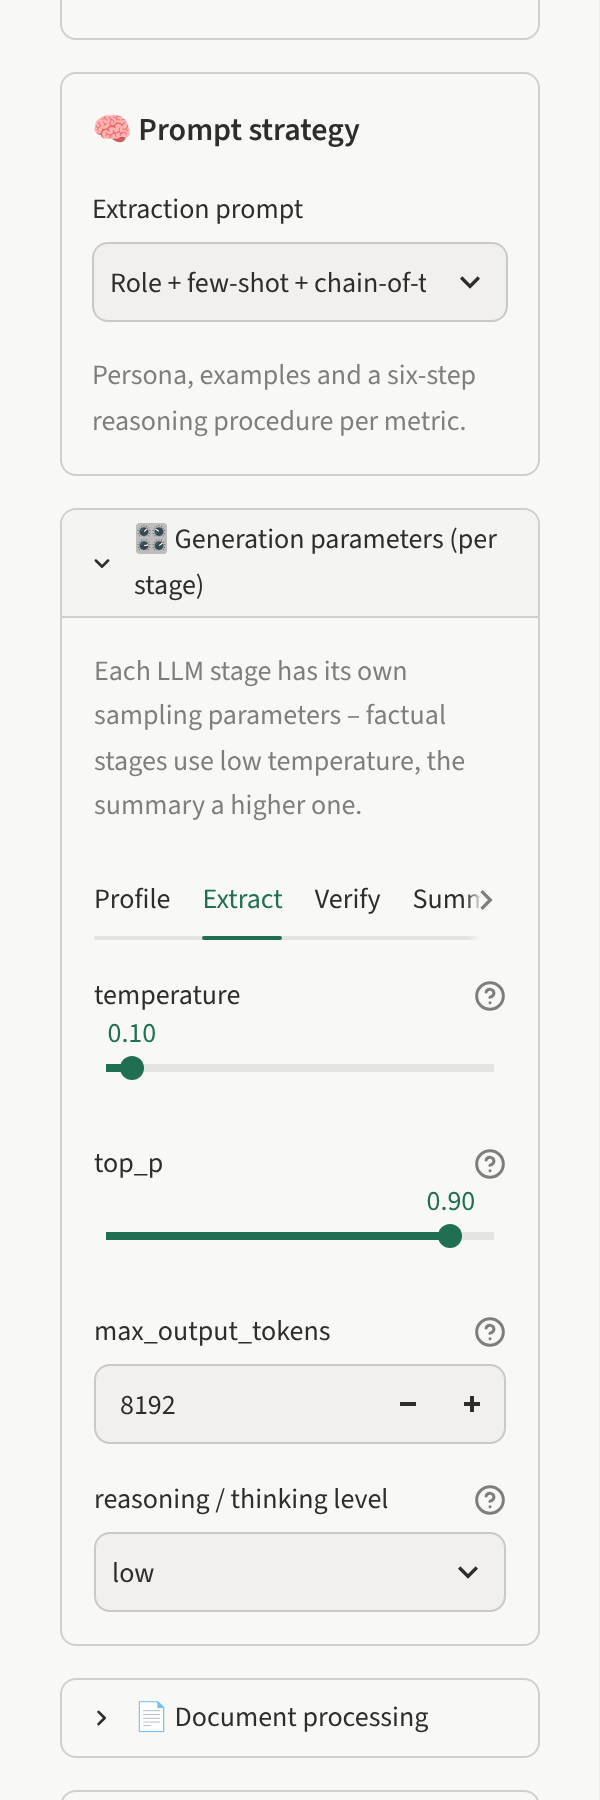
\includegraphics[width=0.92\linewidth]{figures/ui_parameters.png}}}{\fbox{\parbox{\linewidth}{\centering figures/ui\_parameters.png}}}
\end{minipage}\hfill
\begin{minipage}[c]{0.68\linewidth}
\caption{Generation parameters in the sidebar. Each LLM stage (Profile, Extract, Verify, Summary) has its own
\code{temperature}, \code{top\_p}, \code{max\_output\_tokens} and reasoning level. The values used are
stored with every LLM call and shown in the \emph{Report \& Pipeline} tab, so every result can be traced
back to the parameters that produced it.}
\label{fig:params}
\end{minipage}
\end{figure}

% =====================================================================
\section{Validation and hallucination control}\label{sec:validation}
\subsection{Rule-based checks}
Every extracted value is checked against the PDF with deterministic rules (\code{validation.py}):
\begin{itemize}
  \item \textbf{page in range} -- the cited page exists;
  \item \textbf{value on page} -- the number appears on the cited page in any common print format
        (41{,}250 / 41\,250 / 41.250), with digit boundaries so that 1{,}250 does not match inside 41{,}250;
  \item \textbf{evidence grounded} -- at least 70\,\% of the words of the quote occur on the page;
  \item \textbf{unit plausible} -- e.g.\ an emissions value must have a mass/CO$_2$e unit;
  \item \textbf{range} -- percentages in $[0,100]$, pay ratios in $(0,3]$, no negative quantities, plausible years;
  \item \textbf{not a target} -- the quote contains no target language (``by 2030'', ``aim to'', ``net zero by'').
\end{itemize}
Text-layer checks are marked not applicable for values read from charts. Units are normalised to the
standard units of the validated database (t\,CO$_2$e, m$^3$, t, MWh, \%), e.g.\ 12.9\,kt\,CO$_2$e $\rightarrow$
12{,}900\,t\,CO$_2$e and 350\,ML $\rightarrow$ 350{,}000\,m$^3$.

\subsection{Fusion into a final status}
\begin{table}[H]
\centering\small
\begin{tabularx}{\linewidth}{@{}lX@{}}
\toprule
\textbf{Status} & \textbf{Condition}\\\midrule
\textcolor{esggreen}{\textbf{VALID}} & verifier \textsc{valid} \emph{and} number and quote found on the page (or chart source) \emph{and} no target language; or, without AI verification, all text checks pass\\
\textcolor{esgamber}{\textbf{UNCERTAIN}} & verifier \textsc{uncertain}; or verifier and PDF disagree (verifier \textsc{valid} but number not on page); or a verifier correction was applied\\
\textcolor{esgred}{\textbf{INVALID}} & verifier \textsc{invalid}, or a hard rule failure (page does not exist, impossible range)\\
\textbf{NOT FOUND} & the extractor reported the metric as not disclosed\\
\bottomrule
\end{tabularx}
\caption{Status logic.}
\end{table}
A verifier's \code{corrected\_value} is accepted only if that number actually appears on the page.
The final confidence combines the three sources:
\begin{equation}
c = 0.40\,c_\text{extractor} + 0.35\,v_\text{verifier} + 0.25\,r_\text{rules},\qquad v\in\{1, 0.5, 0\},\ r=\text{share of passed checks}.
\end{equation}

% =====================================================================
\section{Error handling}\label{sec:errors}
Error handling is layered: input validation, a provider-independent error taxonomy with retries, recovery
strategies in the pipeline, and a UI that never crashes.

\begin{table}[H]
\centering\small
\begin{tabularx}{\linewidth}{@{}>{\raggedright\arraybackslash}p{4.1cm}>{\raggedright\arraybackslash}p{3.6cm}X@{}}
\toprule
\textbf{Situation} & \textbf{Detection} & \textbf{Response}\\\midrule
Not a PDF, empty, $>$80\,MB, corrupt, encrypted & header check, PyMuPDF open, \code{needs\_pass} & clear message, no API call\\
Single pages unreadable & exception per page & page skipped, warning, analysis continues\\
Scanned document & no text layer, large image & pages sent as images, warning\\
Missing / invalid API key & before the run; HTTP 401/403, ``API key not valid'' & Analyze button disabled with instructions; \code{AuthenticationError}, run stops\\
Rate limit (429 per minute) & status code, message & exponential backoff with jitter (2, 4, 8\,s \ldots), honours \code{retry-after} / ``retry in 17.5s''\\
Daily quota exhausted & 429 + ``per day'' & no pointless retries; advice to switch model/provider\\
Timeout, 5xx, connection error & SDK exception type, status & retried up to 4 times\\
Prompt too large (413, context length) & status / message & context budget halved, one image dropped, retried (twice)\\
Unsupported parameter & 400 mentioning the parameter & retried once without optional parameters\\
Malformed / truncated JSON & local parser, Pydantic & local repair $\rightarrow$ model self-repair (shorter output if truncated)\\
Groq JSON-mode failure & 400 \code{json\_validate\_failed} & the failed generation is repaired\\
Repetitive output at low $T$ & repeated tail substring & extraction retried at $T=1.0$\\
Model omits / duplicates metrics & schema post-processing & missing $\rightarrow$ not found; duplicates $\rightarrow$ best one kept\\
Profiling / verification / summary fails & exception in stage & graceful degradation, result marked \emph{partial}\\
Unexpected error in one view & try/except per tab & error box in that tab, other tabs keep working\\
\bottomrule
\end{tabularx}
\caption{Error handling.}
\end{table}

The retry loop is shared by both providers:
\begin{lstlisting}[style=py]
def call_with_retries(provider, request, max_attempts=4, on_event=None, sleep=time.sleep):
    for attempt in range(1, max_attempts + 1):
        try:
            response = provider.generate(request)
            response.attempts = attempt
            return response
        except LLMError as error:
            if not error.retryable or attempt == max_attempts:
                raise                      # auth, quota, bad request: fail fast
            wait = error.retry_after or backoff_delay(attempt)   # server hint first
            on_event(f"{type(error).__name__} -> retrying in {wait:.0f}s")
            sleep(min(wait, 90))
\end{lstlisting}
Every retry is shown live in the progress log, and every call is stored with its attempts, latency, tokens
and status.

% =====================================================================
\section{User interface}\label{sec:ui}
The Streamlit interface has a settings sidebar and eight tabs:
\begin{description}[style=nextline,leftmargin=1.2cm]
  \item[Analyze] upload or load the fictional sample report, see the plan (number of calls, model,
        strategy), run with a live progress bar and log, KPIs.
  \item[ESG Metrics] disclosure completeness per pillar, status chart, filterable metric table with
        standardised values and confidence, time series of earlier years, downloads.
  \item[Evidence] ``Where did this number come from?'': value card, quote, extractor reasoning, rule checks,
        verifier verdict and the PDF page rendered with the value highlighted.
  \item[Summary] executive summary, E/S/G paragraphs, strengths, gaps, red flags, follow-up.
  \item[Report \& Pipeline] report profile, page statistics, retrieved pages with BM25 scores and matched
        metrics, every LLM call with parameters, tokens, latency and attempts.
  \item[Prompt Lab] experiments (Section~\ref{sec:experiments}) and the prompt inspector.
  \item[History] analyses from SQLite (reopen, delete) and token usage per model and stage.
  \item[About] pipeline overview and links to the free API keys.
\end{description}

\screenshot{ui_start.png}{Analyze tab with the sample report selected. The sidebar holds provider, model,
API key and prompt strategy; the yellow box is the missing-key check, which disables the Analyze button
before any API call is made.}{fig:start}
\screenshot{ui_metrics.png}{ESG Metrics tab after analysing a report with Gemini.}{fig:metrics}
\screenshot{ui_evidence.png}{Evidence tab: the value, its quote, the checks and the highlighted source page.}{fig:evidence}
\screenshot[0.95\linewidth]{ui_promptlab.png}{Prompt Lab with the prompt inspector showing the exact system instruction and user prompt.}{fig:lab}

% =====================================================================
\section{Persistence, file management and exports}\label{sec:storage}
Each analysis is saved in a SQLite database (\code{data/esg\_intelligence.db}) with three tables:
\code{analyses} (one row per analysis with counts per status and the full result as JSON),
\code{llm\_calls} (stage, provider, model, temperature, top\_p, max tokens, reasoning level, tokens,
latency, attempts, status) and \code{experiments} (Prompt Lab runs). Uploaded PDFs are stored once under
\code{data/uploads/<sha256>.pdf}; when the same file is uploaded again, the app offers to load the previous
result instead of spending free-tier quota. Results can be exported as an Excel workbook (metrics, time
series, profile, summary, LLM calls, retrieved pages, warnings), CSV, JSON and a Markdown briefing.

% =====================================================================
\section{Experiments: the Prompt Lab}\label{sec:experiments}
\subsection{Method}
To isolate the effect of the prompt, the report is parsed, profiled and retrieved \emph{once}; then only the
extraction call is repeated for every combination of prompt strategy $\times$ temperature $\times$ repeat.
Each run is scored automatically:
\begin{itemize}
  \item \textbf{Found} -- metrics reported as found;
  \item \textbf{Grounded} -- share of found (text/table) values whose number appears on the cited page;
  \item \textbf{Evidence} -- share whose quote appears on the cited page;
  \item \textbf{JSON first try} -- output valid without self-repair;
  \item \textbf{Stability} -- share of metrics with identical values across repeats (effect of temperature);
  \item \textbf{Agreement} -- share of metrics with the same value as the reference configuration;
  \item \textbf{Accuracy} -- if ground truth is supplied: share of reference values matched within 1\,\%
        (after unit normalisation);
  \item latency and tokens.
\end{itemize}
Ground truth can be any CSV/Excel file with metric ID, year and value columns -- including the validated
database of the earlier project (\code{Metric ID}, \code{Reporting Year}, \code{Validated Value}).
For the bundled fictional sample report a ground-truth file with 15 values is provided
(\nolinkurl{samples/northwind_ground_truth.csv}). The sample is built to be difficult: water consumption
appears \emph{only} in a bar chart, and it contains a 2030 emissions target, a 2028 diversity target,
a Scope~3 category, total waste next to recycled waste, a GHG intensity, a table of contents, a GRI index
and a scanned (image-only) page.

\subsection{Experiments}
\begin{enumerate}
  \item[E1] \textbf{Prompt strategy ablation} -- the four strategies of Table~\ref{tab:strategies} at the
        default temperature, on the sample report (accuracy available) and on one real report.
  \item[E2] \textbf{Temperature and stability} -- the default strategy at $T\in\{0, 0.5, 1.0\}$ with three
        repeats each.
  \item[E3] \textbf{Multimodal effect} -- the default configuration with and without page images
        (sidebar switch); the chart-only water value is the indicator.
  \item[E4] \textbf{Cross-model verification} -- verification with the same model vs.\ a Groq model; the
        number of \textsc{uncertain}/\textsc{invalid} values is compared.
\end{enumerate}
Hypotheses: few-shot examples reduce target/category confusions (higher accuracy and grounding);
chain-of-thought decomposition helps most on multi-year tables; low temperature increases stability; page
images are necessary for chart-only values.

\subsection{Results}
The Prompt Lab exports its results as a ready-made LaTeX table (button ``prompt\_lab\_results.tex''). Upload
it to the folder \code{results/} of this Overleaf project and it appears below automatically.

\IfFileExists{results/prompt_lab_results.tex}{\input{results/prompt_lab_results.tex}}{%
\begin{center}\fcolorbox{esggreen}{esggreen!4}{\parbox{0.86\linewidth}{\centering\small
\textbf{Results table to add:} run the Prompt Lab in the app (e.g.\ all four strategies, temperatures 0 and 1,
with \texttt{samples/northwind\_ground\_truth.csv} as ground truth), download
\texttt{prompt\_lab\_results.tex} and upload it to \texttt{results/} in Overleaf.}}\end{center}}

\textbf{Discussion.} \emph{(Write 4--6 sentences after running the experiments: which strategy had the highest
accuracy and grounding, whether the zero-shot baseline extracted targets or Scope~3 categories, how stable
the results were at $T=0$ vs.\ $T=1$, whether the chart-only value was found with and without images, and
what the cost in tokens and latency was.)}

% =====================================================================
\section{Testing}\label{sec:tests}
The project contains 57 automated tests (\code{pytest}) that run without an API key, using an offline
test double that answers each stage with simple rules and can be scripted to raise errors.

\begin{table}[H]
\centering\small
\begin{tabularx}{\linewidth}{@{}lX@{}}
\toprule
\textbf{Area} & \textbf{Examples of what is tested}\\\midrule
JSON parsing & fences, \code{<think>} tags, trailing commas, truncated output detection, bare lists\\
Schemas & number formats (12,345 / 1.234,5 / (120)), fiscal years, confidence words, dropped bad history points\\
PDF & invalid, empty and encrypted files; scanned-page detection; page limit warning\\
Retrieval & emissions and board pages ranked first; chart page selected for images; context budget\\
Validation & unit normalisation, number boundaries, hallucinated value caught, target language, status fusion, verifier corrections\\
LLM client & error classification (Gemini and Groq SDK errors), retry then success, fail-fast on auth, retries exhausted\\
Pipeline & full run, self-repair, context shrinking, auth stop, profile/verification degradation, unparseable output\\
Storage \& exports & SQLite round trip, Excel/CSV/Markdown, Prompt Lab scoring, LaTeX export, ground-truth file\\
\bottomrule
\end{tabularx}
\caption{Automated tests (all passing).}
\end{table}
In addition, the user interface was exercised end to end in a headless browser (all tabs, analysis,
Prompt Lab), and real requests to both APIs were sent with an invalid key to confirm that the request format
is accepted and that the authentication error is classified correctly.

% =====================================================================
\section{Limitations and future work}
\begin{itemize}
  \item \textbf{Free-tier limits.} Daily request quotas restrict large experiments; the app minimises calls
        (4 per report, caching by file hash) but cannot remove the limits.
  \item \textbf{Lexical retrieval.} BM25 misses pages that use unusual wording; embeddings or a re-ranker could
        help. Scanned documents are only covered through the first page images.
  \item \textbf{Chart reading.} Values read from charts cannot be checked against the text layer and are
        therefore at most \textsc{valid} through the verifier, often \textsc{uncertain}.
  \item \textbf{One report at a time.} The metric set is fixed to 17 (+4) indicators and one reporting year.
\end{itemize}
The application is designed as phase~1 of a larger system: a database of companies and years, an agent that
detects missing company--year combinations, finds and downloads the reports, runs this pipeline and writes
verified values into PostgreSQL. A systematic comparison of text-only RAG, multimodal RAG and multimodal RAG
with agent verification (accuracy, evidence correctness, missing-value handling, hallucination rate and cost)
against the validated database is a natural next step.

% =====================================================================
\section{Conclusion}
ESG Report Intelligence shows that generative AI can do substantive document work when it is embedded in a
pipeline: retrieval narrows the input, carefully engineered prompts (persona, examples, decomposition,
structured output) guide extraction, deterministic rules and an independent auditor prompt check every
value against the source, and the user can see exactly where each number came from. Parameters are chosen
per task and the Prompt Lab turns prompt engineering into a measurable experiment. The application runs
on free APIs, handles the typical failures of real-world AI services, and stores and exports its results
for further use.

% =====================================================================
\begin{thebibliography}{99}\small
\bibitem{csrd} European Parliament and Council. Directive (EU) 2022/2464 (Corporate Sustainability Reporting Directive). \emph{Official Journal of the EU}, 2022.
\bibitem{esrs} European Commission. Delegated Regulation (EU) 2023/2772 -- European Sustainability Reporting Standards (ESRS), 2023.
\bibitem{ghg} WRI and WBCSD. \emph{The Greenhouse Gas Protocol: A Corporate Accounting and Reporting Standard}, revised edition, 2004.
\bibitem{gri} Global Reporting Initiative. \emph{GRI Standards}. \url{https://www.globalreporting.org/standards/}
\bibitem{rag} P.~Lewis et al. Retrieval-augmented generation for knowledge-intensive NLP tasks. \emph{NeurIPS}, 2020.
\bibitem{bm25} S.~Robertson and H.~Zaragoza. The probabilistic relevance framework: BM25 and beyond. \emph{Foundations and Trends in Information Retrieval}, 3(4), 2009.
\bibitem{fewshot} T.~Brown et al. Language models are few-shot learners. \emph{NeurIPS}, 2020.
\bibitem{cot} J.~Wei et al. Chain-of-thought prompting elicits reasoning in large language models. \emph{NeurIPS}, 2022.
\bibitem{selfrefine} A.~Madaan et al. Self-Refine: Iterative refinement with self-feedback. \emph{NeurIPS}, 2023.
\bibitem{nucleus} A.~Holtzman, J.~Buys, L.~Du, M.~Forbes and Y.~Choi. The curious case of neural text degeneration. \emph{ICLR}, 2020.
\bibitem{gemini3} Google. Gemini 3 developer guide and model documentation. \url{https://ai.google.dev/gemini-api/docs/gemini-3}, accessed November 2026.
\bibitem{groq} Groq. API documentation: models, vision, reasoning and rate limits. \url{https://console.groq.com/docs}, accessed November 2026.
\bibitem{pymupdf} Artifex. PyMuPDF documentation. \url{https://pymupdf.readthedocs.io}
\bibitem{streamlit} Streamlit documentation. \url{https://docs.streamlit.io}
\end{thebibliography}

% =====================================================================
\appendix
\section{Running the application}
\begin{enumerate}
  \item Create a free Gemini key at \url{https://aistudio.google.com/apikey} (optionally a Groq key at
        \url{https://console.groq.com/keys}).
  \item On Windows double-click \code{run\_app.bat}: it creates a virtual environment, installs the packages,
        opens \code{.env} for the key and starts the app at \url{http://localhost:8501}.
  \item Manually: run \code{pip install -r requirements.txt}, copy \code{.env.example} to \code{.env} and add the key; then run
        \code{streamlit run app.py}. Tests: \code{python -m pytest -q}.
\end{enumerate}

\section{Metric catalogue}
\begin{longtable}{@{}rlll@{}}
\toprule
\textbf{ID} & \textbf{Metric} & \textbf{Pillar} & \textbf{Standard unit}\\\midrule\endhead
8 & Scope 1 GHG emissions total & E & t CO$_2$e\\
9 & Scope 2 GHG emissions total (market- or location-based noted) & E & t CO$_2$e\\
10 & Scope 3 GHG emissions total & E & t CO$_2$e\\
33 & Waste diverted from disposal: total reused/recycled & E & t (or \%)\\
48 & Water discharge: percentage returned that is purified & E & \%\\
50 & Water consumption: total & E & m$^3$\\
69 & Maternity leave fully covered & S & \%\\
70 & Paternity leave fully covered & S & \%\\
73 & Women in leadership & S & \%\\
75 & Women in management & S & \%\\
80 & Women-to-men average salary ratio: leadership & S & ratio\\
83 & Women-to-men average salary ratio: management & S & ratio\\
86 & Women-to-men average salary ratio: workforce & S & ratio\\
89 & Suppliers with forced or compulsory labour violations & S & count\\
90 & Suppliers with child labour violations & S & count\\
71 & Women on board & G & \%\\
77 & Women-to-men average salary ratio: board & G & ratio\\\midrule
101 & Total energy consumption (extended) & E & MWh\\
102 & Renewable electricity share (extended) & E & \%\\
103 & Total employees (extended) & S & count\\
104 & Lost-time injury frequency rate (extended) & S & rate\\
\bottomrule
\end{longtable}

\section{Code structure}
\begin{table}[H]
\centering\small
\begin{tabular}{@{}ll@{}}
\toprule
\textbf{File} & \textbf{Responsibility}\\\midrule
\code{app.py} & Streamlit user interface\\
\code{esg\_intel/config.py} & providers, models, default parameters, metric catalogue\\
\code{esg\_intel/pdf\_processor.py} & validation, text/table/visual extraction, rendering, highlights\\
\code{esg\_intel/retrieval.py} & BM25 ranking, image page selection, context builder\\
\code{esg\_intel/prompts.py} & all prompts and the four prompt strategies\\
\code{esg\_intel/llm\_client.py} & Gemini and Groq clients, error taxonomy, retries\\
\code{esg\_intel/schemas.py} & Pydantic schemas with tolerant coercion\\
\code{esg\_intel/json\_utils.py} & robust JSON parsing\\
\code{esg\_intel/validation.py} & rule checks, unit normalisation, status fusion\\
\code{esg\_intel/pipeline.py} & end-to-end pipeline, self-repair, graceful degradation\\
\code{esg\_intel/experiments.py} & Prompt Lab runs, scoring, LaTeX export, ground truth\\
\code{esg\_intel/storage.py} & SQLite database and PDF file store\\
\code{esg\_intel/export.py} & Excel, CSV, JSON, Markdown exports\\
\code{esg\_intel/mock\_provider.py} & offline test double\\
\code{tests/} & 57 automated tests\\
\code{samples/} & fictional sample report, its generator and ground truth\\
\bottomrule
\end{tabular}
\caption{Project files.}
\end{table}

\end{document}
